% --- Folie 2: Forschungsfrage ---
\begingroup
\frametitle{Fraunhofer AISEC}
\begin{frame}
	\begin{figure}
		\centering
		\includegraphics[width=0.7\linewidth]{BilderPräsentation/AISEC.png}
		\caption{Fraunhofer-Institut in Garching}
		\label{fig:enter-label}
	\end{figure}
	\vspace{0.2em}
	\begin{itemize}
		\item Fraunhofer-Institut für Angewandte und Integrierte Sicherheit in Garching
		\item Cognitive Security Technologies
		\begin{itemize}
			\item Künstliche Intelligenz und IT-Sicherheit
		\end{itemize}
	\end{itemize}
\end{frame}
\endgroup


\begingroup
\frametitle{Motivation}
\begin{frame}
	\begin{itemize}
		
		\uncover<1->{
			\item[] Neuronale Netze dominieren viele Bereiche:
			\item[]
			{\scriptsize
				\begin{tabular}{@{}p{0.45\textwidth}@{\hspace{1.4em}}p{0.45\textwidth}@{}}
					\hspace{1.4em}
\includegraphics[height=1em]{BilderPräsentation/image.png} Bildverarbeitung &
					
\includegraphics[height=1em]{BilderPräsentation/alert.png} Anomalieerkennung \\
					\hspace{1.4em}
\includegraphics[height=1em]{BilderPräsentation/text.png} Textverarbeitung &
					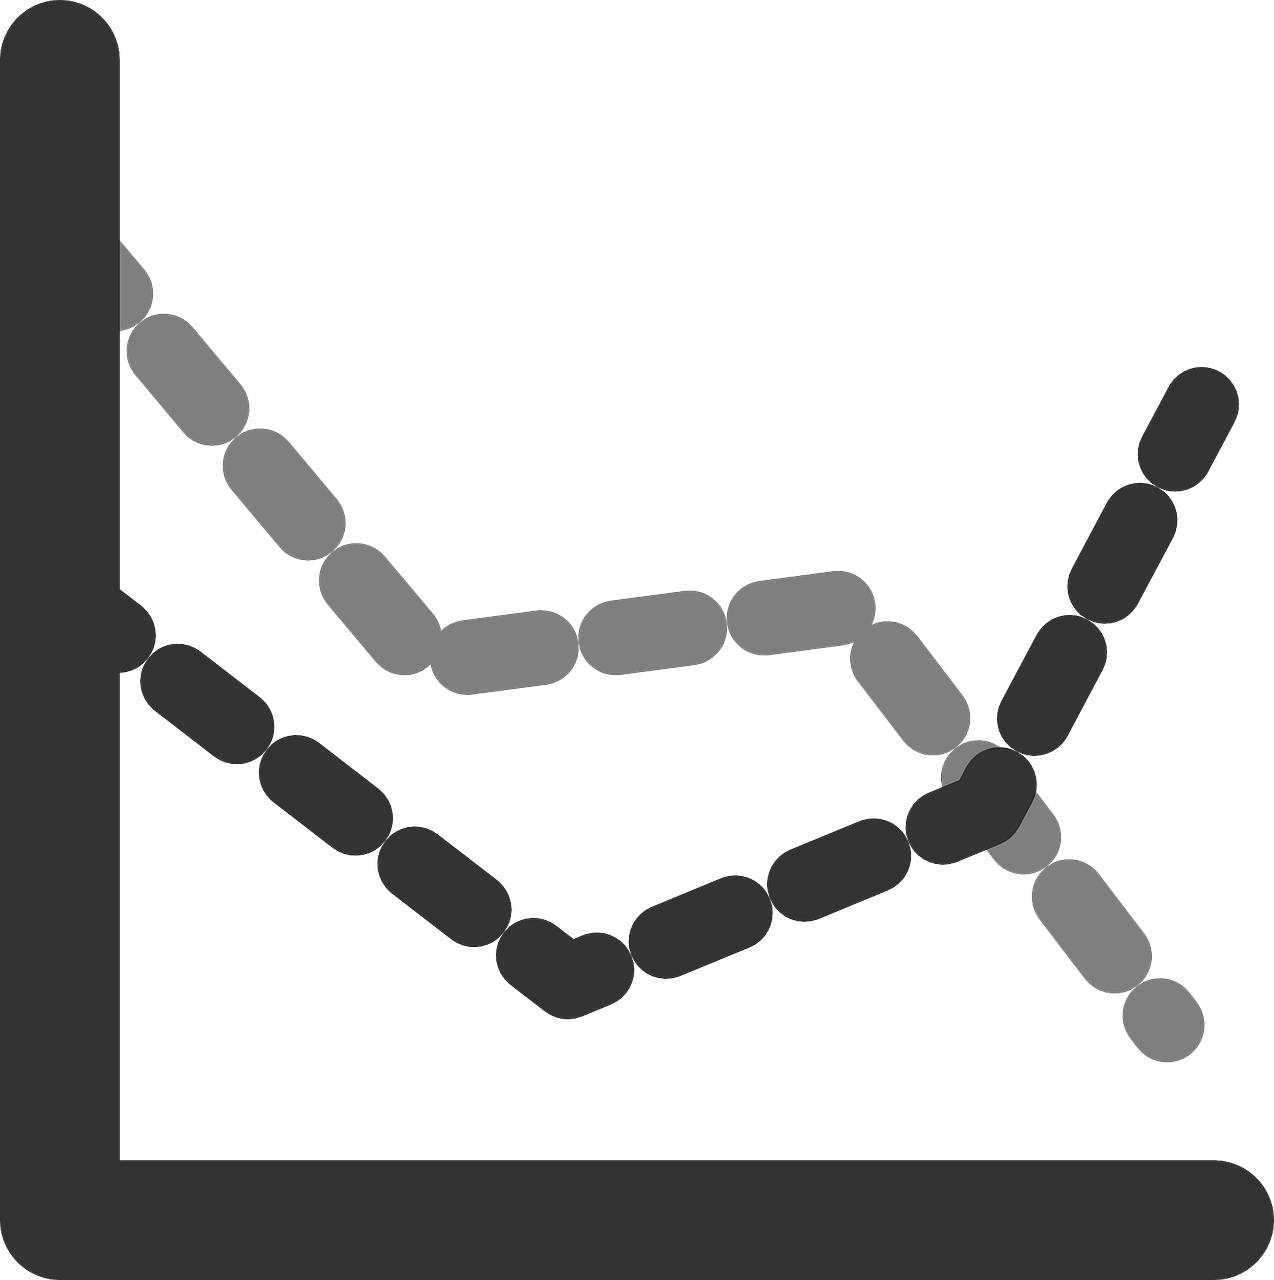
\includegraphics[height=1em]{BilderPräsentation/predict.png} Klassifikation und Vorhersage
				\end{tabular}
		}}
		
		\vspace{0.4em}
		
		\uncover<1->{
			\item[] 
\includegraphics[height=1em]{BilderPräsentation/network.png} Sie lernen komplexe, nichtlineare Funktionen~\cite{antiga_deep_2020}}
		
		\vspace{0.4em}
		
		\uncover<2->{
			\item[] 
\includegraphics[height=1em]{BilderPräsentation/question.png} Wie ähnlich sind zwei Netze?
			\begin{itemize}
				\item Verständnis interner Repräsentationen
				\item Gleiche Architektur
				\item Unterschiedliches Training
		\end{itemize}}
		
	
		
	\end{itemize}
	{\tiny Quelle: Antiga et al., “Deep Learning with PyTorch”, Manning 2020~\cite{antiga_deep_2020}}
\end{frame}
\endgroup

\begingroup
\frametitle{Forschungsansatz}
\begin{frame}
\begin{itemize}
    \item \textbf{Ausgangspunkt}: Chan et al.~\cite{chan_affine_2024} schlagen einen Homotopie-basierten Ansatz zur Modellvergleichbarkeit vor:
    \begin{itemize}
      \item \textbf{Intrinsic Homotopy:} Wie gut kann eine Repräsentation in eine andere transformiert werden?
      \item \textbf{Extrinsic Homotopy:} Wie ähnlich ist das Modellverhalten bei gleichem Downstream-Task?
    \end{itemize}
    
    \vspace{0.8em}
    \item \textbf{Limitation}: Nur \emph{affine} Transformationen $\Rightarrow$ begrenzte Ausdruckskraft für komplexe Modelle.
    \end{itemize}
\vfill
{\tiny Quelle: Chan et al., “On Affine Homotopy between Language Encoders”, NeurIPS 2024~\cite{chan_affine_2024}}
\end{frame}
\endgroup

\begingroup
\frametitle{Forschungsfragen}
\begin{frame}
\vspace{0.8em}
\textbf{Forschungsfragen:}
\begin{itemize}
  \item Wie lassen sich intrinsic und extrinsic Homotopy im nichtlinearen Fall definieren?
  \item Erfassen nichtlineare Transformationen Ähnlichkeit besser als lineare?
  \item Besteht ein konsistenter Zusammenhang zwischen intrinsic und extrinsic Homotopy?
\end{itemize}
\end{frame}
\endgroup

